\section{Vorversuche}
\label{Vorversuche}
Um einen Eindruck über den zu erwartenden Datensatz und Schwierigkeiten zu erhalten, wurde einige Testdatensätze mit der Actioncam erstellt.\\
\subsection{Arbeitsbereich der Verfahren - Versuch 1}
Mit diesem Versuch soll der Zusammenhang zwischen Standort der Probanden und Targets untersucht werden. Dazu wird ein Klassenzimmer simuliert mit weit verteilten Schüler, die den gesamten frontalen Betrachten.
\subsubsection{Versuchsaufbau}
In einem Raum wurde die Kamera in $2.06m$ Höhe $31cm$ hinter den Targets so montiert, das der gesamte Raum im Fokus liegt. Als Targets wurden 9 Punkte auf einer Ebene markiert mit der Kamera im Zentrum. Die Anordnung der Targets ist in \autoref{img_aufbau_target_Test} dargestellt.\\
Als Position der Probanden wurde ein Rastfeld mit $1m$ Kantenlänge im Raum eingezeichnet auf einer Fläche von $7 \times 11m$. Die Probanden stellten sich auf diesen Positionen auf um nacheinander alle Targets zu Betrachten. 
\begin{figure}
	\centering
	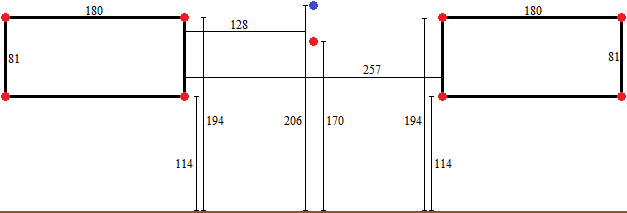
\includegraphics[width=0.7\linewidth]{PositionWinkel/Target}
	\caption{Aufbau der Targets im Vorversuch, alle Angaben gerundet in Zentimeter\\rote Punkte: Target, blauer Punkt: Kamera}
	\label{img_aufbau_target_Test}
\end{figure}
\subsubsection{Detektion mit MTCNN}
Um die Detektionswahrscheinlichkeit der MTCNN-Face Detektor zu testen wurden dieses Videos analysiert.\\
Es zeigt sich, das auf allen Positionen die Probanden erfolgreich erkannt wurden und die Boxen das Gesicht recht gut beschreibt. Allerdings ist zu erkennen, das die Landmarks unzureichend genau sind. Sie sollten die Mundwinkel, Nasenspitze und beide Augen markieren, liegen aber schon bei recht großen Bilder weit daneben, siehe \autoref{img_bereich_MTCNN}
\subsubsection{Auswertung}
Für die Analyse wurde aus dem Video jene Frames ausgewählt in denen ein Target fokussiert wurde und Analysiert.\\
Für eine Analyse wurde zuerst die Einzelbildauswertung von OpenFace auf die Frames angewendet und jene resultierende Kopfrotationen markiert, an denen eine erfolgreich ein Gesicht erkannt wurde. In \autoref{graph_Test_Bilder} ist der horizontale Wertebereich dargestellt in denen an der jeweiligen Position ein Gesicht erfolgreich erkannt wurde.\\
Im zweiten Teil wurden die selben Frames für die Messung verwendet, dieses mal allerdings wurde das gesamte Video analysiert. Der Winkelbereich in denen auf der horizontalen Achse an den entsprechenden Positionen ein Gesicht erkannt wurde, ist in \autoref{graph_Test_Video} dargestellt.\\
Das Fehlen von Ergebnissen in Spalte $-3m$ liegt an der unzureichenden Detektion. Als Ursache kann die Überbeleuchtung durch das einfallende Licht der Fenster angenommen werden. 
\begin{figure}
	\centering
	\begin{tabular}{|c|c|c|c|c|c|}
		\hline 
		$+5m$ & &
		
\includegraphics[width=1.4cm]{PositionWinkel/Winkel_-100_500.png} &
		
\includegraphics[width=1.4cm]{PositionWinkel/Winkel_0_500.png} &
		
\includegraphics[width=1.4cm]{PositionWinkel/Winkel_100_500.png} & \\ 
		\hline 
		$+4m$ & 
\includegraphics[width=1.4cm]{PositionWinkel/Winkel_-200_400.png} &
		
\includegraphics[width=1.4cm]{PositionWinkel/Winkel_-100_400.png} &
		
\includegraphics[width=1.4cm]{PositionWinkel/Winkel_0_400.png} &
		
\includegraphics[width=1.4cm]{PositionWinkel/Winkel_100_400.png} &
		
\includegraphics[width=1.4cm]{PositionWinkel/Winkel_200_400.png} \\ 
		\hline 
		$+3m$ & 
\includegraphics[width=1.4cm]{PositionWinkel/Winkel_-200_300.png} & 
\includegraphics[width=1.4cm]{PositionWinkel/Winkel_-100_300.png} & 
\includegraphics[width=1.4cm]{PositionWinkel/Winkel_0_300.png} & 
\includegraphics[width=1.4cm]{PositionWinkel/Winkel_100_300.png} & 
\includegraphics[width=1.4cm]{PositionWinkel/Winkel_200_300.png} \\ 
		\hline 
		$+2m$ & 
\includegraphics[width=1.4cm]{PositionWinkel/Winkel_-200_200.png} &
		
\includegraphics[width=1.4cm]{PositionWinkel/Winkel_-100_200.png} &
		
\includegraphics[width=1.4cm]{PositionWinkel/Winkel_0_200.png} &
		
\includegraphics[width=1.4cm]{PositionWinkel/Winkel_100_200.png} & \\ 
		\hline 
		$+1m$ & &
		
\includegraphics[width=1.4cm]{PositionWinkel/Winkel_-100_100.png} &
		
\includegraphics[width=1.4cm]{PositionWinkel/Winkel_0_100.png} &
		
\includegraphics[width=1.4cm]{PositionWinkel/Winkel_100_100.png} & \\ 
		\hline 
		& $-2m$ & $-1m$ &Kamera& $+1m$ & $+2m$ \\ 
		\hline 
	\end{tabular}
	\caption{Dargestellt ist der horizontale Winkebereich in dem mit der Image-Verarbeitung ein Gesicht erkannt wurden.}
	\label{graph_Test_Bilder}
\end{figure}
\begin{figure}
	\centering
	\begin{tabular}{|c|c|c|c|c|c|c|}
		\hline
		$+5m$ &
		
\includegraphics[width=1.4cm]{PosWinkelVideo/Winkel_V_200_500.png}&
		
\includegraphics[width=1.4cm]{PosWinkelVideo/Winkel_V_100_500.png}&
		
\includegraphics[width=1.4cm]{PosWinkelVideo/Winkel_V_0_500.png}&
		
\includegraphics[width=1.4cm]{PosWinkelVideo/Winkel_V_-100_500.png}&
		
\includegraphics[width=1.4cm]{PosWinkelVideo/Winkel_V_-200_500.png}&
		
\includegraphics[width=1.4cm]{PosWinkelVideo/Winkel_V_-300_500.png}\\ 
		\hline 
		$+4m$ &
		
\includegraphics[width=1.4cm]{PosWinkelVideo/Winkel_V_200_400.png}&
		
\includegraphics[width=1.4cm]{PosWinkelVideo/Winkel_V_100_400.png}&
		
\includegraphics[width=1.4cm]{PosWinkelVideo/Winkel_V_0_400.png}&
		
\includegraphics[width=1.4cm]{PosWinkelVideo/Winkel_V_-100_400.png}&
		
\includegraphics[width=1.4cm]{PosWinkelVideo/Winkel_V_-200_400.png}&
		
\includegraphics[width=1.4cm]{PosWinkelVideo/Winkel_V_-300_400.png}\\ 
		\hline 
		$+3m$ &
		
\includegraphics[width=1.4cm]{PosWinkelVideo/Winkel_V_200_300.png}&
		
\includegraphics[width=1.4cm]{PosWinkelVideo/Winkel_V_100_300.png}&
		
\includegraphics[width=1.4cm]{PosWinkelVideo/Winkel_V_0_300.png}&
		
\includegraphics[width=1.4cm]{PosWinkelVideo/Winkel_V_-100_300.png}&
		
\includegraphics[width=1.4cm]{PosWinkelVideo/Winkel_V_-200_300.png}&
		
\includegraphics[width=1.4cm]{PosWinkelVideo/Winkel_V_-300_300.png}\\ 
		\hline 
		$+2m$ & &
		
\includegraphics[width=1.4cm]{PosWinkelVideo/Winkel_V_100_200.png}&
		
\includegraphics[width=1.4cm]{PosWinkelVideo/Winkel_V_0_200.png}&
		
\includegraphics[width=1.4cm]{PosWinkelVideo/Winkel_V_-100_200.png}&
		
\includegraphics[width=1.4cm]{PosWinkelVideo/Winkel_V_-200_200.png} &\\ 
		\hline 
		$+1m$ & &
		
\includegraphics[width=1.4cm]{PosWinkelVideo/Winkel_V_100_100.png}&
		
\includegraphics[width=1.4cm]{PosWinkelVideo/Winkel_V_0_100.png}&
		
\includegraphics[width=1.4cm]{PosWinkelVideo/Winkel_V_-100_100.png}& &\\ 
		\hline 
		& $-2m$ & $-1m$ &Kamera& $+1m$ & $+2m$ & $+3m$ \\ 
		\hline 
	\end{tabular}
	\caption{Dargestellt ist der horizontale Winelbereich in dem mit der Video-Verarbeitung ein Gesicht erkannt wurde.}
	\label{graph_Test_Video}
\end{figure}
\subsubsection{Ergebnis}
Es zeigt sich, dass eine Auswertung auf einem Video deutlich zuverlässiger arbeitet als auf Einzelbilder, vor allem der größere Rotationsbereich ist von Vorteil.\\
Durch die Verwendung des Weitwinkelobjektivs, kann die gesamte Breite eines Klassenzimmers erfasse werden und der Winkelbereich für eine erfolgreiche Detektion ist breit genug um Schüler erfassen zu können, die selbst die fordern Eckpunkte eines Klassenzimmers betrachten.\\
Bei der Distanz zur Kamera (Tiefe) ist Handlungsbedarf, als Ziel wurde $8m$ angesetzt und das aktuelle Verfahren endet bei $5m$.\\
Eine signifikante Aussage bezüglich des vertikalen Winkel kann aus diesem Aufbau nicht getroffen werden, da die Neigungswinkel zu ähnlich ausfallen bei stehenden Personen und beide einem geradeaus Blick ähneln.
\subsection{Arbeitsbereich der Verfahren - Versuch 2}
Da ein aufmerksamer Schüler durchaus auch auf den Tisch blicken kann, z.B. beim Schreinen, so soll getestet werden wie weit die Analyse in solchen Situationen funktioniert.
\subsubsection{Versuchsaufbau}
Für diesen Versuch wurde die Kamera auf $1.88m$ Höhe und $3m$ vor den vordersten Standort der Probanden aufgestellt.\\
Als Standorte wurde eine Markierung mit einem Meter Abstand zueinander auf eine Gerade bei $3m$ und $9m$ verwendet.\\
Als Target diente die Kamera, ein Punkt $78cm$ unterhalb der Kamera und einer $40cm$ über dem Boden und $50cm$ vor der Kamera. Alle anderen Targets befinden sich $1m$ vor den Standorten.\\
Diesmal war das Versuchsgelände draußen an einem bedecken Tag, wodurch eine helle schattenlose Szene entsteht.
\subsubsection{Auswertung}
ToDo
\subsubsection{Ergebnisse}
Es zeigt sich, das eine Videoanalyse auch bei starke Neigung nach unten möglich ist. Die Einzelbildauswertung liefert erneut deutlich schlechter Ergebnisse als des Videos.\\
Dabei funktioniert das Traking nur, wenn die Versuchsperson zuerst in die Kamera geschaut hat, um es zu beginnen. Auch die stärkere gleichmäßige Beleuchtung ist hilfreich, da die Problematik mit Gegenlicht und Schatten entsteht.
\subsection{Auswertung der Augenpartie - Versuch 3}
Um einen Eindruck von ElSe mit hochauflösenden Aufnahmen zu erhalten, wurde mit einer Fotokamera (Sony ILCE-6000, Farbbild $6000\times 4000$ Pixel, Brennweite $16mm$) an den selben Positionen wie in Versuch 1 ein weiterer Datensatz von Einzelbilder erstellt, dabei wurden nur Aufnahmen mit der Kamera als Target gemacht. Von Interesse ist die Augenpartie und die Ergebnisse des OpenFace Eye-Detektor im Vergleich zu ElSe.\\
Dabei wurde ElSe in der Basis Konfiguration eingesetzt, dies bedeutet das Luminance-Verfahren, siehe \autoref{gray_Luminance} als Graukonvertierer und einem Radius der Maske von 12 Pixel.
\subsubsection{Auswertung}
Für die Analyse wurde zuerst mit OpenFace das Gesicht soweit analysiert um die Augenpartie als Eingabebild zu bestimmen, siehe \autoref{graph_Auge_Verbesserung} und ein Beispiel in \autoref{img_Versuch_Auge} oben. Auf diesem Eingabebild wird nun der ElSe-Algorithmus angewendet um die Ellipse zu bestimmen, dargestellt in grün. Im Vergleich sind die zusätzlichen 28 Landmarks der Augen von OpenFace auch in \autoref{img_Versuch_Auge} Mitte oben. Als Ergebnis wurde aus den berechneten Ellipse von ElSe die Landmarks der Pupille und Iris abgeleitet und im selben Farbschema dargestellt.\\
Die einzelnen Augenpaare stammen von der selben Person, die sich bei der angegebenen Distanz frontal vor der Kamera befand. Es ist zu erkennen, das selbst bei einer hohen Auflösung die Augenpartie sehr klein ausfällt und nur schwierig auszuwerten ist.
\begin{figure}
	\centering
	\begin {tikzpicture}
	\node[draw,align=center] (in) at(0,0) {Eingabebild\\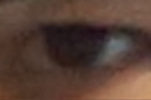
\includegraphics[width=0.18\linewidth]{img_Versuch_Auge/Auge_in}};
	\node[draw,align=center] (El) at(6,0)  {Ellipse\\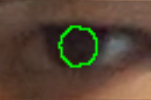
\includegraphics[width=0.18\linewidth]{img_Versuch_Auge/Auge_EL}};
	\node[draw,align=center] (OF) at(6,-4) {Landmark\\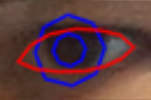
\includegraphics[width=0.18\linewidth]{img_Versuch_Auge/Auge_OF}};
	\node[draw,align=center] (ER) at(12,0)  {Ergebnis\\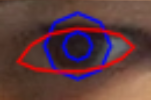
\includegraphics[width=0.18\linewidth]{img_Versuch_Auge/Auge_ER}};
		
	\draw[->] (in)to node[above]{ElSe}(El);
	\draw[->] (in)to node[left]{OpenFace}(OF);
	
	\draw[->] (El)to node[above]{Iris \& Pupille}(ER);
	\draw[->] (OF)to node[right]{Augenlider}(ER);	
\end{tikzpicture}
	\caption{Dargestellt sind der Ablauf, um die Landmarks des Auges zu verbessern}
	\label{graph_Auge_Verbesserung}
\end{figure}
\begin{figure}
	\centering
	\begin{tabular}{|c|c|c|c|c|c|c|c|c|c|c|} 
		\hline 
		\includegraphics[width=0.07\linewidth]{img_Versuch_Auge/Auge_2}&
		\includegraphics[width=0.07\linewidth]{img_Versuch_Auge/Auge_3}&
		\includegraphics[width=0.07\linewidth]{img_Versuch_Auge/Auge_6}&
		\includegraphics[width=0.07\linewidth]{img_Versuch_Auge/Auge_7}&
		\includegraphics[width=0.07\linewidth]{img_Versuch_Auge/Auge_10}&
		\includegraphics[width=0.07\linewidth]{img_Versuch_Auge/Auge_11}&	
		\includegraphics[width=0.07\linewidth]{img_Versuch_Auge/Auge_14}&
		\includegraphics[width=0.07\linewidth]{img_Versuch_Auge/Auge_15}&
		\includegraphics[width=0.07\linewidth]{img_Versuch_Auge/Auge_17}&
		\includegraphics[width=0.07\linewidth]{img_Versuch_Auge/Auge_19}&
		\includegraphics[width=0.07\linewidth]{img_Versuch_Auge/Auge_22}\\
		\hline 
		$1m$&$2m$&$3m$&$4m$&$5m$&$6m$&$7m$&$8m$&$9m$&$10m$&$11m$\\ 
		\hline 
	\end{tabular}
	\caption{Ergebnisse von OpenFace und ElSe bei verschiedenen Distanz.\\ Von Oben nach Unten: Augenparie, Ergebnis OpenFace, Ergebnis ElSe, ElSe Ergebnis als Landmarks}
	\label{img_Versuch_Auge}
\end{figure}
\subsubsection{Ergebnis}
Es zeigt sich das trotz einer hohen Bildauflösung der Informationsgehalt auf größere Distanzen deutlich abnimmt, wenn mit einer einzigen Kamera der gesamte Bereich einer Klasse erfasst werden soll. Außerdem ist auch gut zu erkennen das eine ausreichende Beleuchtung gebracht wird, da die Augenregion sehr dunkel ausfällt.
\subsection{Ergebnis der Vorversuche}
Es zeigt sich das der Arbeitsbereich in Hinblick auf Rotationen ausreichend ist um alle üblichen Bewegungen eines Schülers zu erfassen. Auch die Fläche auf dem sich die Schüler verteilen können ist vielversprechend, nur die Distanz muss noch verbessert werden.\\
Auch MTCNN-Face ist als Detektor geeignet, er findet zuverlässige alle Gesichter im Frame, unabhängig ihrer Größe und Orientierung. Sogar jene die von OpenFace auch bei der Videoanalyse nicht verwendbar sind. Einzige Anmerkung ist die etwas ungenaue Box, dies kann aber mit einer einfachen Verschiebung der Boxränder korrigiert werden.